\documentclass[../document.tex]{subfiles}
\begin{document}
\section{Model}
This section gives an high level overview of the steps in our approach. We will first describe the data gathering,  then the post processing pipeline used to generate the dataset. After, we will introduced the model used to fit the data and then show the results with different test environments.
\subsection{Robot: Krock}
Our task was to apply the approach proposed in \cite{omar@traversability} with a legged robot developed at EPFL named 
\emph{Krock}. Figure \ref{fig:krock} shows the robot in the simulated environment.
\begin{figure}[H]
    \centering
    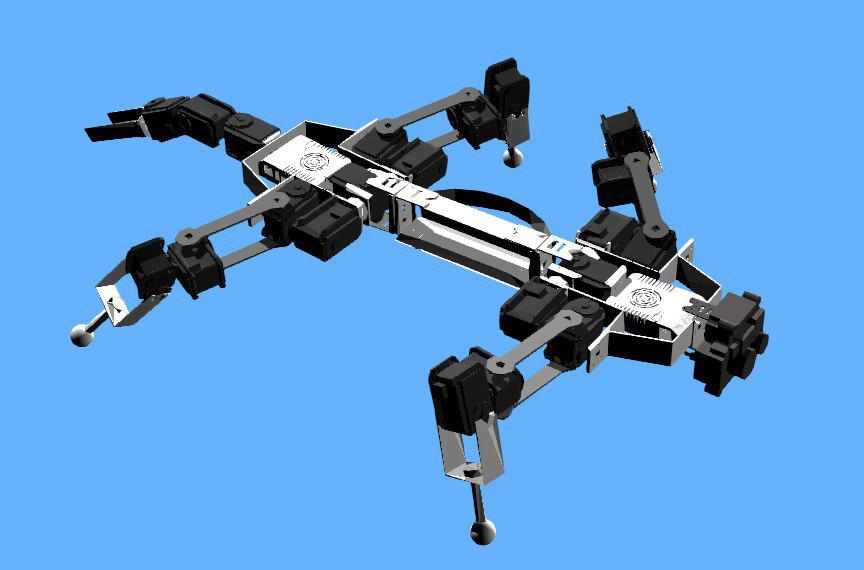
\includegraphics[width=0.5\linewidth]{img/krock-1.jpg}
    \label{fig:krock}
    \caption{\emph{Krock}}
\end{figure}
Krock has four legs, each one of them is equipped with three motors in order to rotate in each axis. The robot is 
also able to rise itself in three different configurations, gait, using the four motors on the body connected 
to the legs. In addition, there are an other set of two motors in the inner body part to increase krock's move set. 
The tail is composed by another set of three motors and can be used to perform a wide array of tasks.
The robot is $85cm$ long and weights around $1.4kg$. The next figure \ref{fig:krock-top} shows \emph{Krock} from the top helping the reader understanding its composition and the correct ratio between its parts. Also, each motor is highlighted with a red marker.
\begin{figure}[H]
\centering
     \begin{subfigure}[b]{0.49\textwidth}
    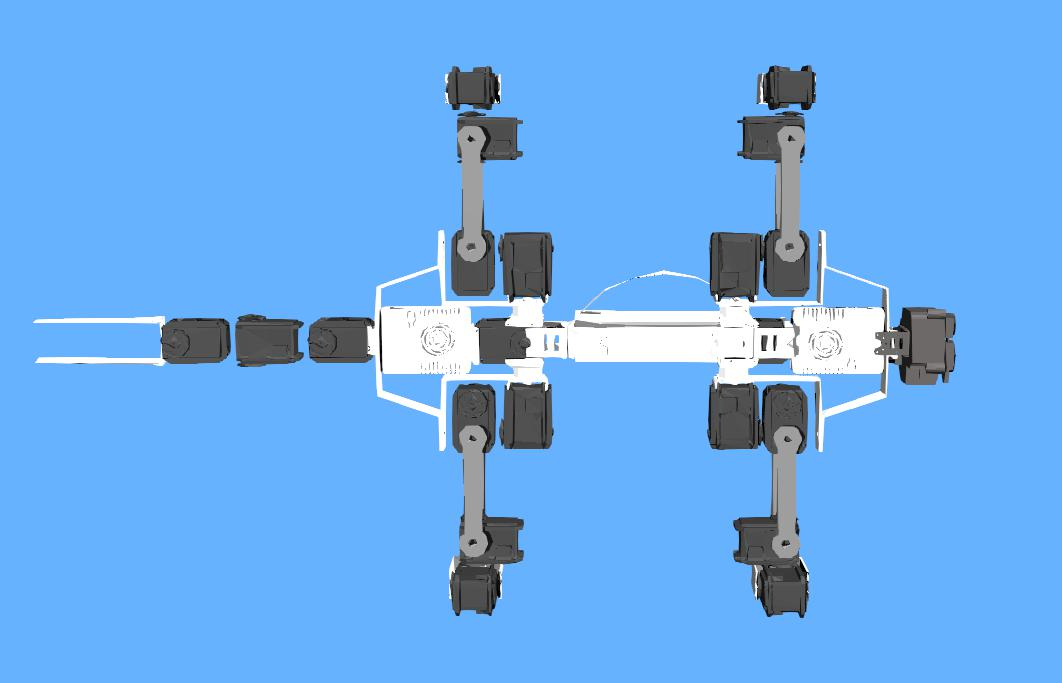
\includegraphics[width=\textwidth]{img/krock-top.jpg}
    \caption{Top view of \emph{Krock}}
   	\end{subfigure}
     \begin{subfigure}[b]{0.49\textwidth}
      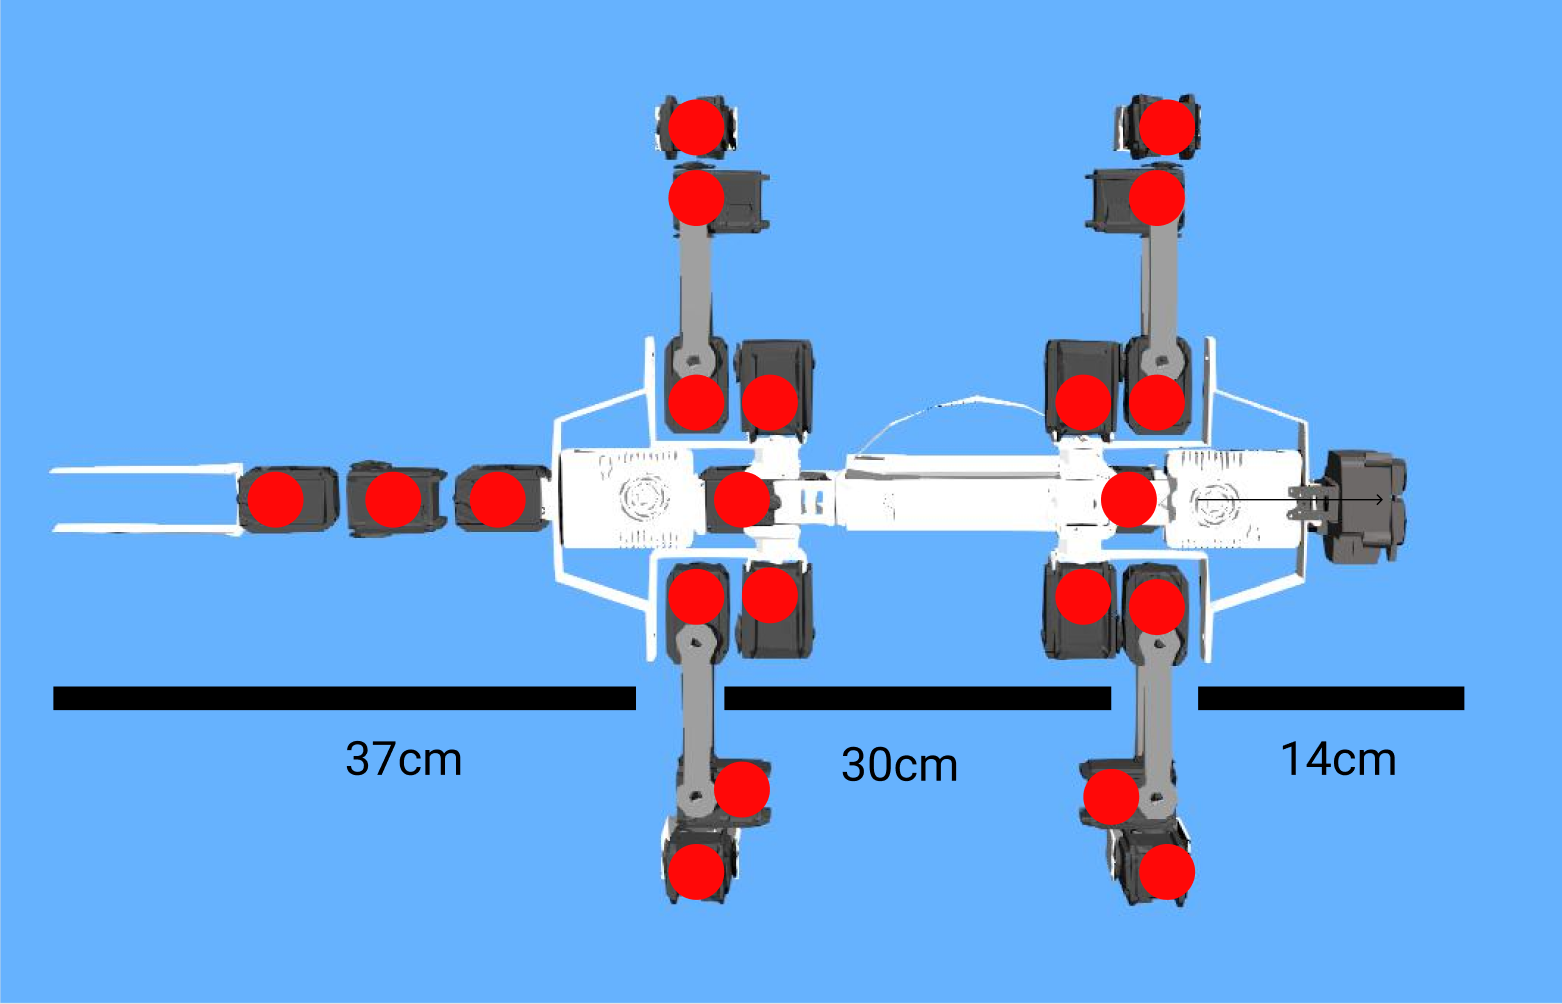
\includegraphics[width=\textwidth]{img/krock-top-highlight.png}
    \caption{Details highlighted in \emph{Krock}}
   	\end{subfigure}
   	    \label{fig:krock-top}

\end{figure}
\emph{Krock}'s moves by lifting and moving forward one leg after the other. The following figure shows the robots going forward.
	\begin{figure}[H]
\centering
    	\begin{subfigure}[b]{0.3\textwidth}
			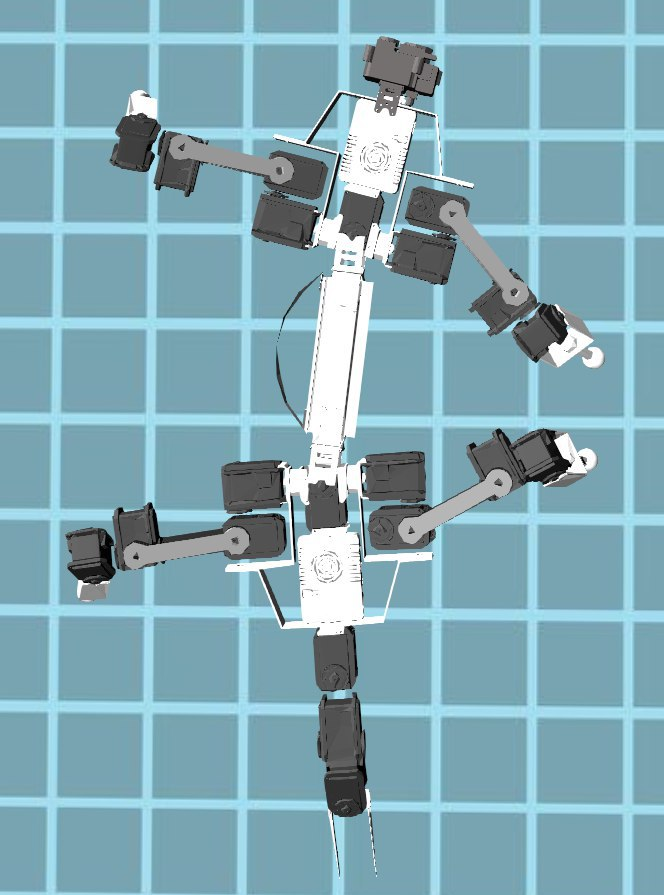
\includegraphics[width=\textwidth]{img/krock-moving-1}
			\caption{$t=1$}
	    \end{subfigure}
		\begin{subfigure}[b]{0.3\textwidth}
			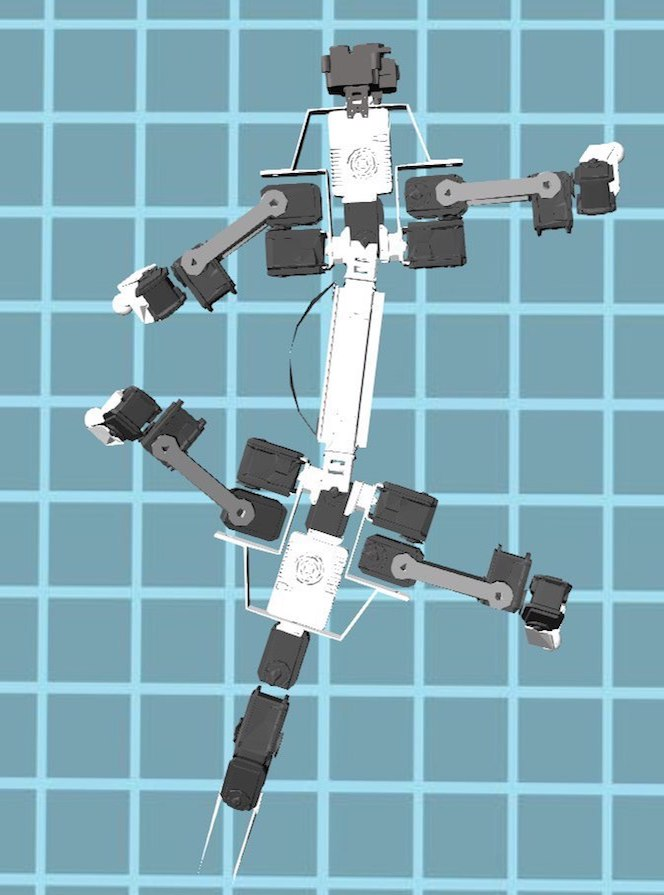
\includegraphics[width=\textwidth]{img/krock-moving-2}
			\caption{$t=2$}
	    \end{subfigure}	
	   \begin{subfigure}[b]{0.3\textwidth}
			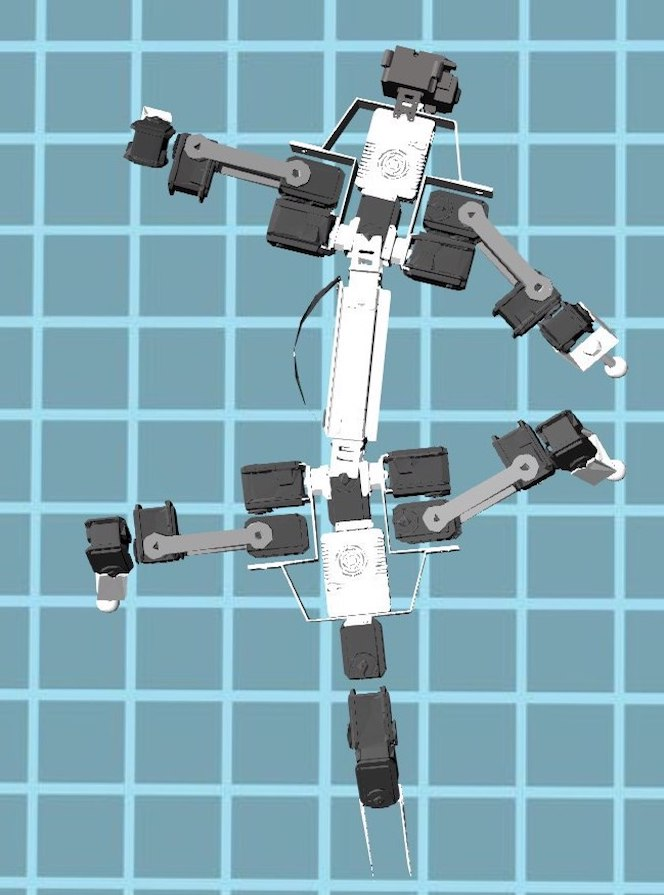
\includegraphics[width=\textwidth]{img/krock-moving-3}
			\caption{$t=3$}
	    \end{subfigure}	
	\label{fig: krock-moving}
	\caption{\emph{Krock} moving forward.}
	\end{figure}
\emph{Krock} can also raise its own body in three different configurations. Figure 

\todo[inline]{Add Krock gait picture}

\begin{figure}
\ref{fig: krock-gait}
\caption{\emph{Krock} differents gait configuration.}	
\end{figure}
\subsection{Simulation}
Our approach relies on simulations to collected the data needed to train the estimator. We used Webots \cite{webots}, a professional 
mobile robot simulator, as backbone for our framework. 

We generate fifteen synthetic $10x10$ meters long heightmaps with different features, such as walls, bumps and slopes using the same techniques described in \cite{omar2018traversability}. Figure \ref{fig:heightmaps}
show some of the maps used in the simulator. 

A heightmap is grey image, formally a 2D array, where each element, pixel, represents a height value. Since each image has a range from $[0,255]$, we also need to scale them when needed. For this reason, we associated a height scaling value for each heightmap that is used to increase or decrease the steepness. 

\todo[inline]{Add heightmap picture}
\todo[inline]{Add heightmap and a 3d render of that map}
\todo[inline]{add two 3d render of a map with two different height values}

\begin{figure}[H]
    \todo[inline]{TODO}
\label{fig:heightmaps}
\caption{Some of the heightmaps used in the simulation.}
\end{figure}

To generate the train data, each map is loaded into the simulator, then the robot is spawned in the world and we let it walked forward for a certain amount of time or until it reaches the edge of the map. While moving, we store his pose, that contains position and orientation, with a rate of $50hz$. 

We fix the robot's gait in its standard configuration and run fifteen simulations for each map, where one simulation one robot spawns and death, with a height scale factor of one. We also decide to include steepest training samples by using one of the maps with a slope with heights factors from $[1,7]$. The following pictures shows this specific map with different scaling factors. 

\todo[inline]{add slope map with different height values}

\emph{Krock} is equipped with a controller implemented with the Robotic Operating System (ROS) software that is used as a communication channel between our framework and the simulator. Basically, ROS exposes nodes, called \emph{topics}, in which we can listen for incoming messages. Thus, \emph{Krock} is able to stream its pose to all the clients connected to its pose topic. 

We also generate the test set, by running the robot in real world environment, such as \emph{Quarry} a cave map, that we later use to test the fitted model. 

\todo[inline]{Add the quarry 3d height map  3d render}

By observing the simulations we notice two problems. First, \emph{Krock}'s tail sometime gets under the body, second, if a random spawn strategy is used, in certain maps the agent may directly fell on an obstacle.

To overcame the first problem, we decide to remove the tail after we ensure by asking to the developers that this will not compromise the traversability. We immediately observe less noisy data. 

\todo[inline]{add krock with and without tail}

The second issue was more challenging. If the robot spawns on an obstacle then it will be stuck for all the simulation compromising the quality of the data. This is very important for the \emph{bars} map, where there are lots of wall of different sizes and the probability to fell on one of them is very high. So, for some maps  we guarantee that \emph{Krock} does not directly spawn into obstacles by only spawning the robot in flat ground first. The following figures shows the result of this strategy on the \emph{bars1} map where the robot was spawned where there are no obstacle.

\todo[inline]{add krock spawns on bars1}

We run a total of \todo{add number of simulations} storing the results using ROS's \emph{.bag} files for a total of \todo{add size of all bags.}.
\section{Postprocessing}
In order to create the training dataset we need to postproces the data stored during the simulation. To train our classifier we need to fist compute the advancement for each pose at each time for a specific time window, $pose_{it}$. Then, we can use it to crop a patch from the heightmap that was used in the simulation of the correct size. Such patch must include the whole \emph{Krock} footprint and the maximum possible advancement in a given time window. 
By keeping this final goal in mind, we quickly describe each step taken to reach it. Figure shows each step applied in the pipeline. 

\todo[inline]{add figure to show our pipeline like with bricks}

We implemented an easy to use API \todo{link to the project} to define a cascade stream of function that are applied one after the other using a multi-thread queue to speed-up the process.
First, we convert each \emph{.bag} file into a \emph{.csv} file and store it since this operation must be done only once. Then, we define a time window $t$ and for each entry in one simulation run we compute the future advancement using booth position and angle from the pose, we also store the resulting Dataframe into a \emph{.csv} file. During the process, we also clean the data by removing the samples in which the robot was upside down or out of the map.

Finally, we crop from each heightmap the patches corresponding to each data point. To compute the patch size need to know the maximum possible advancement of \emph{Krock} for a specific time window. In order to find it, we run \emph{Krock} on a flat ground map and we take the mean across all of them. We observer a mean advancement of $33cm$ per second.

For a given advancement, we ensure the whole \emph{Krock} footprint is included on the left part to take into account the situations in which an obstacle is directly under the robot. To clearly show the process, we used a simulated environment in which \emph{krock} has a big wall in front of him and one small under his legs. The following picture shows the terrain.

\todo[inline]{add figure with the two walls}

Clearly, assuming \emph{Krock} is able to traverse $33$cm of flat ground per second, in one second it won't be able to reach the obstacle, this is shows in the first picture. Increasing the time window, the taller wall appears while the small one under the robot is always correctly included.


\todo[inline]{add figure with the patch computation}

\section{Estimator}
At this point, we have a dataset composed of patches and the corresponding advancement. Obliously, to perform classification we need classes, thus we must label each patch as \emph{traversable} or \emph{not traversable}. To archieve it, we selected a treshold, $tr$, and labeled each patch by $patch_{advancement} > tr$. In other words, if \emph{Krock} was able to advance in a patch more than the treshold, then that patch is label as \emph{traversable} and viceversa. The pair patches and labels represent the final dataset.

We used a deep convolutional neural network to fit the training set. Convolutional Neural Network are able to learn patterns into images and map them to target classes. 
Before feeding the patches into the model, we subtract in each patch the value in the middle in order to normalise them by making height invariant.
\end{document}
